% !TEX root = main.tex

\begin{proof}[Proof of Claim~\ref{cl:infix}]
Fix a  one-turn \slps $\Lambda=\alpha_1\beta_1^*\alpha_2\beta_2^*$, and
let $M:=\size(\Lambda)$ and $S_2 := R(S_1)$.
Our goal is to show that the set $S_2 = \bigcup_{c\in S_1} R(\{c\})$
%For $c \in S_1$ let us denote $R(c) = \set{v_2 \in (u_1, c) \tran (v_1, v_2)}$.
%Let $R(S_1) = \bigcup_{c \in S_1} R(c)$. Our goal is to show that $R(S_1)$ 
is a finite union
of $(a', r', T')$-arithmetic sequences for $a' \leq a + \poly(B, M, r)$ and $r' \leq \poly(M)$.
We write $R(c)$ instead of $R(\{c\})$.

Let $\eff(\beta_1) = (x_1, -y_1)$ and $\eff(\beta_2) = (-x_2, y_2)$, for some $x_1, x_2, y_1, y_2 \in \Npos$.
% (recall that $\beta_1$
%and $\beta_2$ belong to the corresponding quadrants by assumptions of Claim~\ref{cl:infix}).
Every path $\rho = \alpha_1\beta_1^{n_1}\alpha_2\beta_2^{n_2}$ is determined by 
a pair $(n_1,n_2) \in \N^2$,
and hence when $(u_1, u_2) \tran (v_1, v_2)$, we may also write $(u_1, u_2) \trans {(n_1,n_2)} (v_1, v_2)$
for $(n_1, n_2)\in\N^2$, or 
$(u_1, u_2) \trans {(n_1,n_2)}$ when the target vector is not relevant.
%and we say that $\rho = \rho(n_1, n_2)$.
Whenever this happens, we necessarily have the equality
%We are interested in possible $c_2 \in \N$ such that there is $c_1 \in S_1$ such that $(b_1, c_1) \trans{(n_1, n_2)} (b_2, c_2)$
%for some $n_1, n_2 \in \N$. Notice that looking at the first coordinate gives the following equation
$
u_1 + \eff_1(\alpha_1 \alpha_2) + n_1 x_1 - n_2 x_2 = v_1
$
of effects on the first coordinate,
which we transform to an equation with two unknowns $n_1,  n_2$:
\begin{equation}\label{eq:xy}
n_1 x_1 - n_2 x_2 = v_1 - u_1 - \eff_1(\alpha_1 \alpha_2).
\end{equation}
%
The set of solutions $(n_1, n_2)$ of~\eqref{eq:xy} is of the form $w+p^*$, 
where $w = (w_1, w_2) \in \N^2$ is the minimal solution of~\eqref{eq:xy}
and $p = (p_1, p_2) \in \N^2$ is the minimal solution of its uniform version, $n_1 x_1 - n_2 x_2 = 0$.
By Lemma~\ref{lem:solutions} we get $\norm(w) \leq \poly(B, M)$. One can easily observe that $\norm(p) \leq 2M$
($(x_1, x_2) = (n_2, n_1)$ is a solution).
%
Let $\eff_2(w) = -w_1 y_1 + w_2 y_2$ and $\eff_2(p) = -p_1 y_1 + p_2 y_2\in \N$ be 
the effects induced by $w$ and $p$, respectively, on the second coordinate.

\begin{example}\label{ex:infix}
\begin{figure}[t]
\vspace{-2cm}
\begin{minipage}{0.5\textwidth}
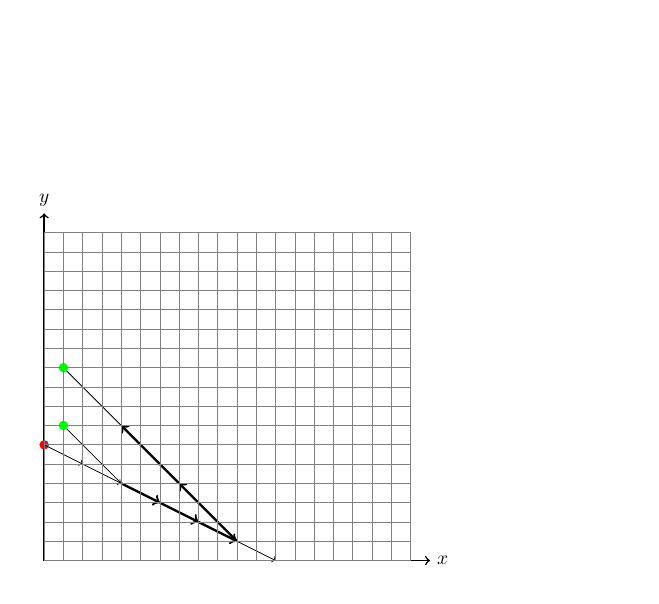
\begin{tikzpicture}[scale=0.35]
\scalebox{0.7}{
\draw[->, thick] (0, 0) -- (20, 0) node[right] {$x$};
\draw[->, thick] (0, 0) -- (0, 18) node[above] {$y$};

\fill[red] (0,6) circle (7pt);

\draw[->] (0,6) -> (2,5);
\draw[->] (2,5) -> (4,4);
\draw[very thick,->] (4,4) -> (6,3);
\draw[very thick,->] (6,3) -> (8,2);
\draw[very thick,->] (8,2) -> (10,1);
\draw[->] (10,1) -> (12,0);

\draw[->] (4,4) -> (1,7);
\fill[green] (1,7) circle (7pt);

\draw[very thick,->] (10,1) -> (7,4);
\draw[very thick,->] (7,4) -> (4,7);
\draw[->] (4,7) -> (1,10);
\fill[green] (1,10) circle (7pt);

\draw[step=1, gray, thin] (0, 0) grid (19, 17);
}
\end{tikzpicture}
\end{minipage}
\begin{minipage}{0.5\textwidth}
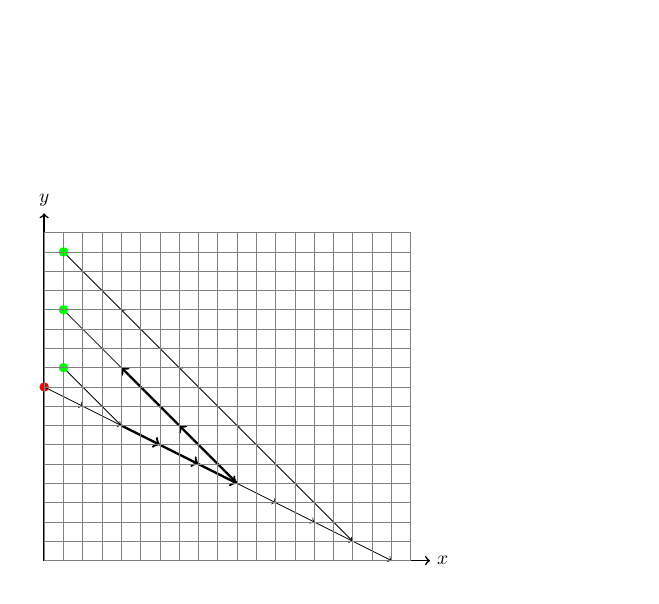
\begin{tikzpicture}[scale=0.35]
\scalebox{0.7}{
\draw[->, thick] (0, 0) -- (20, 0) node[right] {$x$};
\draw[->, thick] (0, 0) -- (0, 18) node[above] {$y$};

\fill[red] (0,9) circle (7pt);

\draw[->] (0,9) -> (2,8);
\draw[->] (2,8) -> (4,7);
\draw[very thick,->] (4,7) -> (6,6);
\draw[very thick,->] (6,6) -> (8,5);
\draw[very thick,->] (8,5) -> (10,4);
\draw[->] (10,4) -> (12,3);
\draw[->] (12,3) -> (14,2);
\draw[->] (14,2) -> (16,1);
\draw[->] (16,1) -> (18,0);

\draw[->] (4,7) -> (1,10);
\fill[green] (1,10) circle (7pt);

\draw[very thick,->] (10,4) -> (7,7);
\draw[very thick,->] (7,7) -> (4,10);
\draw[->] (4,10) -> (1,13);
\fill[green] (1,13) circle (7pt);

\draw[->] (16,1) -> (13,4);
\draw[->] (13,4) -> (10,7);
\draw[->] (10,7) -> (7,10);
\draw[->] (7,10) -> (4,13);
\draw[->] (4,13) -> (1,16);
\fill[green] (1,16) circle (7pt);

\draw[step=1, gray, thin] (0, 0) grid (19, 17);
}
\end{tikzpicture}
\end{minipage}

\caption{Left: $u_2 = 6$, $S_2 = \set{7,10}$. Right: $u_2 = 9$, $S_2 = \set{10,13,16}$.
Thick vectors add up to $p$.}
\label{fig:infix}
\end{figure}

Let $\alpha_1$ and $\alpha_2$ be empty sequences, $\eff(\beta_1) = (2, -1)$ and $\eff(\beta_2) = (-3, 3)$.
Let $u_1 = 0$, $v_1 = 1$. 
The set of solutions $(n_1, n_2)$ of~\eqref{eq:xy} is of the form $w+p^*$, where
$w = (2,1)$ and $p = (3,2)$, and
$\eff_2(p) = 3 \cdot (-1) + 2 \cdot 3 = 3$.
Figure~\ref{fig:infix} shows $R(u_2) = \set{7,10}$ when $u_2 = 6$, and $R(u_2)  = \set{10,13,16}$ when $u_2 = 9$.
In the latter case, elements of $R(u_2)$ correspond to the solutions $w$, $w+p$ and $w+2p$ of~\eqref{eq:xy},
i.e., to $w + kp$ for $k$ in an interval $[0,2]$.
According to Claim~\ref{cl:interval}, this is true in general.
%$S_2 = \setof{u + kp}{k\in I}$, for some interval $I$.
\end{example}

%The following claim states that the number of possible periods $p$ used in the run is an interval.

\begin{claim}\label{cl:interval}
For each $c \in S_1$ there exists an interval $I_{c} = [k_1, k_2]$, where $k_1\in \N$ and $k_2 \in \N_{\infty}$,
such that
$R(c) = \setof{\eff_2(w) + k \cdot \eff_2(p)}{k\in I_{c}}$.
% and path $\rho(b+kp)$ starting from $(b_1, c)$ is a valid if and only if $k \in I_c$. 
\end{claim}

\begin{proof}
It is sufficient to show that whenever $(u_1, c) \trans{w + k_1 \cdot p}$ and
$(u_1, c) \trans{w + k_2 \cdot p}$ for some
$k_1 < k_2 \in \N$,
then
$(u_1, c) \trans{w + k \cdot p}$ for all $k \in [k_1, k_2]$.
Fix $k \in [k_1, k_2]$.
Every point $x$ on the (possibly $\Z$-)path $(u_1, c) \trans{w + k \cdot p}$ is actually on a straight line between some two points,
one on the path $(u_1, c) \trans{w + k_1 \cdot p}$, and the other on the path $(u_1, c) \trans{w + k_2 \cdot p}$.
In consequence $x$, being a weighted average of the two points in $\N^2$, necessarily belongs to $\N^2$. 
Therefore $(u_1, c) \trans{w + k \cdot p}$ is a path.
\end{proof}

We notice that $\eff_2(p)$ can be negative, but this is irrelevant for our arguments.
%
By Claim~\ref{cl:interval}, for each $c \in S_1$ the set $R(c)$ is
is an arithmetic sequence of difference $\essdvass r := \absv{\eff_2(p)}$ and length equal to the cardinality
of the interval $I_{c}$.
%Thus $R(c) = b + (\essdvass r)^{\card{I_c}}$, for some $b\in\N$. 
Let $\spn(c)\in\N_\infty$ be the difference between the supremum of $R(c)$ and the minimal element in $R(c)$.
We say that $\spn(c) = \infty$ if $R(c)$ is infinite.
We split the proof into cases, depending on
whether $\essdvass r$ divides the difference $r$ of the sequence $S_1$, or not.
Additionally we have a case when $\essdvass r = 0$, in other cases we silently assume that $\essdvass r \neq 0$.


\para{Case I: $r$ is divisible by $\essdvass r$}

Therefore, if $\spn(c) \geq r$ then the sequence $R(c)$ actually touches the sequence $R(c+r)$,
i.e., their union is a larger arithmetic sequence of difference $\essdvass r$:

\begin{claim}\label{cl:merged}
If $R(c+r^*) \neq \emptyset$ and $c \geq D:= 3(M+r) \cdot M^2 + M \cdot \norm(w)$,
then $R(c+r^{\leq T}) = b+(\essdvass r)^{\leq T'}$ for some $b \leq c + \eff_2(w) + M \cdot \eff_2(p)$ and $T' \in \N_\infty$.
\end{claim}

\begin{proof}
We first show that $\spn(c) \geq r$.
Suppose $R(c+r^*) \neq \emptyset$ and $c \geq D$.
Due to the first assumption,  for some $n\in\N$ there is a path $(u_1, c+nr) \trans{(n_1, n_2)}$
of the form
\begin{align} \label{eq:Mp}
(u_1, c+nr) \trans{\alpha_1} (\essdvass{x}_1, \essdvass{y}_1) \trans{\beta_1^{n_1}} (\essdvass{x}_2, \essdvass{y}_2) \trans{\alpha_2} (\essdvass{x}_3, \essdvass{y}_3) \trans{\beta_2^{n_2}} (v_1, v_2).
\end{align}
In particular,  $u_1 \geq \drop_1(\alpha_1)$
and therefore $\essdvass x_1\geq 0$.
It is enough to take $(n_1, n_2) := w + Mp$ in \eqref{eq:Mp}.
Then $n_1 \geq M$, so $\essdvass x_2 \geq \essdvass x_1 + M \geq M \geq \drop_1(\alpha_2)$.
Therefore $\essdvass x_3\geq 0$.
Now we show that $c$ is large enough such that $(u_1, c) \trans{w+Mp}$ is nonnegative on the second coordinate as well.
As $\norm(p) \leq 2M$ then $n_1 + n_2 \leq M \cdot \norm(p) + \norm(w) \leq 2M^2 + \norm(w)$. Therefore
$\beta_1^{n_1}$ and $\beta_2^{n_2}$ can in total decrease the second coordinate by at most $M \cdot (2M^2 + \norm(w))$.
As $\alpha_1 + \alpha_2$ can in total decrease the second coordinate by at most $M$ and
$D \geq M + M \cdot (2M^2 + \norm(w))$ we conclude that indeed the path $(u_1, c) \trans{w+Mp}$ is valid.
For the same reasons, for every $m\in [M, M+r]$ there is a path $(u_1, c) \trans{w+mp}$, which guarantees $\spn(c) \geq r$. 

Now we use that fact that $\spn(c) \geq r$.
By monotonicity of \vass, if $R(c) = b+(\essdvass r)^{\leq {T'}}$
then $R(c+r)$ necessarily includes $R(c) + r= b+r+(\essdvass r)^{\leq {T'}}$.
Since $\spn(c) \geq r$, we have $b+r \in R(c)$, but also $b+r \in R(c+r)$,
and therefore the union $R(c) \cup R(c + r)$ forms one arithmetic sequence 
$b+(\essdvass r)^{\leq T'}$, for some $b\in\N$ and $T'$.
The similar reasoning applies to any finite union, namely to $R(c+r^{\leq m})$ for $m\in\N$.
In consequence, for every $T\in \N_\infty$ we have $R(c+r^{\leq T}) = b + (\essdvass r)^{\leq T'}$,
for some $b\in\N$ and $T'\in \N_\infty$,
and since $c+ \eff_2(w) + M \cdot \eff_2(p) \in R(c)$ we get the inequality $b \leq c + \eff_2(w) + M \cdot \eff_2(p)$, as required.
\end{proof}

We are ready for concluding Case I.
%Let $D = 3(M+r) \cdot M^2 + M \cdot \norm(w)$, as in the Claim~\ref{cl:bigspan}.
As $\norm(w) \leq \poly(B, M)$ we have $D \leq \poly(B, M, r)$.
We  partition $S_1 = a + r^{\leq T}$ into two subsets: $S'_1 = S_1 \cap [0,D)$
and $S''_1 = S_1 \cap [D,\infty)$, both being arithmetic sequences of difference $r$,
and consider $S'_1$ and $S''_1$ separately.
 
Concerning $S'_2:= R(S'_1)$,
as $\max(S'_1) \leq D$, all
elements of $S'_2$ are upper-bounded by a polynomial in $M$ and $r$, namely
$\max(S'_2) \leq M^2 \cdot (2M + D)$. 
Thus $S'_2$ can be seen as a finite sum of singletons, each of which
being an $(a', r', T')$-arithmetic sequence with $a' \leq M^2 \cdot (2M + D) \leq \poly(B,M,r)$,
$r' = 1$ and $T' = 0$. 
Clearly $r' = 1 \leq \poly(M)$, and hence $S'_2$ is of the required form.

Now we consider $S''_2:= R(S''_1)$.
If $S''_2 = \emptyset$ we are done.
Otherwise, let $c:= \min(S''_1)$.
Thus $S''_1 = c+r^{\leq T}$ for some $T \in \N_\infty$, 
and $D\leq c \leq \max(a, D+r)$.
%By Claim~\ref{cl:bigspan}, $\spn(c) \geq r$, and therefore using Claim~\ref{cl:neighbours} 
By Claim~\ref{cl:merged} we deduce that
$S''_2 = b + (\essdvass r)^{\leq T'}$ for some 
$b \leq c + \eff_2(w) + M \cdot \eff_2(p)$ and $T' \in \N_\infty'$. 
As $\eff_2(w) \leq \poly(B,M)$, $\eff_2(p) \leq \poly(M)$ and $c \leq a + \poly(B,M, r)$ we get $b \leq a + \poly(B, M, r)$.
We also have $\essdvass r \leq \poly(M)$, and hence
$S''_2$ is of the required form.


\para{Case II: $r$ is not divisible by $\essdvass r$}
%Assume now that $r$ does not divide $\eff_2(p)$. 

In that case we split $S_1 = a + r^{\leq T}$ into several
arithmetic sequences of difference $r \cdot \essdvass r$, namely into sequences of a form 
$(a + m \cdot r) + (r \cdot \essdvass r)^{\leq T'}$, where $m < \essdvass r$, 
and apply the above reasoning to each of this sequences separately. 
As $\essdvass r \leq \poly(M)$
we get also a finite set of arithmetic sequences with the base bounded by $a + \poly(B, M,r)$ and difference bounded by $\poly(M)$,
as required.

\para{Case III: $\essdvass r = 0$}
\Wlog we assume $R(S_1) \neq \emptyset$. For every $c \in S_1$ we have that either $R(c) = c + \eff_2(w)$ or $R(c) = \emptyset$. By monotonicity of VASS we have that if $R(c) \neq \emptyset$ then $R(c+r) \neq \emptyset$. Let $D := 3(M+r) \cdot M^2 + M \cdot \norm(w)$. Similarly as in the proof of Claim~\ref{cl:merged} we observe that if $c \geq D$ then for some $k \in N$ there is a run $(u_1, c) \trans{w+kp}$. Hence we have $R(S_1) = c + \eff_2(w) + r^{\leq T'}$ for some $T' \in \N_\infty$ and some $c \in S_1$ such that $c \leq \max(a, D+r)$. Therefore $R(S_1) = b + r^{\leq T'}$ for some $b \leq a + \poly(B,M,r)$ as required.

\end{proof}



%
%Observe, that if $(b_1, s) \trans \rho (b_2, t)$ for $s \in S_1$ and $t \in S_2$ then $x,y$ satisfy the following equation:
%$$\eff_1(\alpha_1\alpha_2) + x\eff_1(\beta_1) + y\eff_1(\beta_2) = b_2-b_1$$
%Hence we have that the set $S$ of such  pairs $(x,y)$ associated is included in set of solutions of the above equation, which can be represented by Lemma~\ref{lem:taming} as $L(B,P)$ for some sets $B, P \subseteq \N^2$ such that $\norm(B) \leq c(M+B)$ and $\norm(P) \leq cM$ for some constant $c \in \N_+$. We show, that $P$ has only one element $p$. This is because the set of solutions of the following equations over $\Q$ is one dimensional vector space and there is nonnegative solution, because of different signs of $\eff_1(\beta_1)$ and $\eff_1(\beta_2)$:
%$$x\eff_1(\beta_1) + y\eff_1(\beta_2) = 0$$
%Hence each path can be represented as $b+kp$ for some $k \in \N$ and $b \in B$ (recall that with each path we associated pair $(x,y)$). Because $B$ is finite and we are interested in a finite union representation it is enough to show that there exists polynomial $R(M)$ such that the set $S_2' =   \{y_2 \mid \exists_{y_1 \in S_1} (b_1, y_1) \trans{b+kp} (b_2, y_2), k \in \N \}$ is a finite union of $(a', r', T')$-arithmetic sets with $a' \leq a + (B+r) \cdot R(M)$ and
%$r' \leq R(M)$.
%
%We have $p=(p_1, p_2)$ and we write $\eff(p)$ for $\eff(\beta_1^{p_1}\beta_2^{p_2})$. Moreover $b = (b_1, b_2)$ and we write $\eff(b+kp)$ for $\eff(\alpha_1\beta_1^{b_1}\alpha_2\beta_2^{b_2}) + k \eff(p)$. First we solve a case when $|\eff_2(p)|$ divides $r$, to which we will reduce the other case. Let $m = \frac{r}{|\eff_2(p)|}$. Moreover, \mywlog we can assume that $S_2' \neq \emptyset$.
%The intuition is that the set $S_2'$ will be a condensing of $S_1$ due to repetitions of $p$ with base point $a'$ moved a bit. In order to conclude the prove we need a few claims. 
%\begin{claim}
%For each $s \in S_1$ there exists interval $I = [k_1, k_2]$ such that $k_1, k_2 \in \N_{\infty}$ and path $b+kp$ starting from $s$ is a valid path if and only if $k \in I$. 
%\end{claim}
%\begin{proof}
%It is enough to show, that if for $k_1 < k_2 \in \N$ we know, that $b+k_1p$ and $b+k_2p$ are valid paths starting from $s$ then for all $k_3 \in [k_1, k_2]$ we have that path $b+k_3p$ is a valid path starting from $s$. Let us fix $k_3 \in [k_1, k_2]$ and let $b=(b_1, b_2), p=(p_1, p_2) \in \N^2$. Recall, that $\eff(\beta_1) \in \N_+ \times \N_-$ and $\eff(\beta_2) \in \N_- \times \N_+$. Hence it is enough to show the following inequalities:
%$$\eff_1(\alpha_1\beta_1^{b_1+k_3p_1}\alpha_2\beta_2^{b_2+k_3p_2}) = \eff_1(\alpha_1\beta_1^{b_1+k_1p_1}\alpha_2\beta_2^{b_2+k_1p_2})$$
%$$\eff_2(\alpha_1\beta_1^{b_1+k_3p_1}) \geq \eff_2(\alpha_1\beta_1^{b_1+k_2p_1})$$
%For the first equality observe, that:
%\begin{align*}
%\eff_1(\alpha_1\beta_1^{b_1+k_3p_1}\alpha_2\beta_2^{b_2+k_3p_2}) & = \eff_1(\alpha_1\beta_1^{b_1+k_1p_1}\alpha_2\beta_2^{b_2+k_1p_2}) 
%+ (k_3-k_1)(p_1\eff_1(\beta_1) + p_2\eff_1(\beta_2)) \\
%& = \eff_1(\alpha_1\beta_1^{b_1+k_1p_1}\alpha_2\beta_2^{b_2+k_1p_2})
%\end{align*}
%The second inequality follows from the fact that:
%$$b_1+k_3p_1 \leq b_1+k_2p_1$$
%\end{proof}
%Let us by $I_x = [k_1^s, k_2^s]$ denote the interval for $x \in S_1$ and by $|I_x| = k_2^s - k_1^s$. Now we split elements of $S_1$ into three groups depending on the properties of the points in $S_1$.
%\begin{claim}\label{clm:split}
%For each $x \in S_1$ at least one of the following holds:
%\begin{itemize}
%\item $x \leq a + 3cM^2(B+r)$
%\item $x$ is the maximal element of $S_1$ and $[0,m] \subseteq I_x$
%\item $[0, m] \subseteq I_x$ and if $b+kp$ is executable from $(b_1,x)$ for $k > m$ than $b+(k-m)p$ is executable from $(b_1,x+m\eff_2(p))$ and $x+m\eff_2(p) \in S_1$. 
%\end{itemize}
%\end{claim}
%\begin{proof}
%Let us take $x \in S_1$ such that  $x > a + 3cM^2(B+r)$. Firstly, we show that $[0, m] \subseteq I_x$. Recall, that $\Lambda$ is one-turn and observe, that for all $k \in \N$ we have:
%$$\eff_1(\alpha_1\beta_1^{b_1}\alpha_2\beta_2^{b_2}) = \eff_1(\alpha_1\beta_1^{b_1}\alpha_2\beta_2^{b_2}) + k(p_1\eff_1(\beta_1) + p_2\eff_1(\beta_2))$$
%Hence, because $S_2$ is not empty we have that all paths $b+kp$ starting from $(b_1, x)$ are valid on the first counter. Hence we only need to deal with the second counter. Now observe, that for each $k \in [0,m]$ we have that maximal decrease of the second counter along path $b+kp$ is at most :
%\begin{align*}
%M + (b_1+kp_1)\eff_2(\beta_1) & \leq M + (c(M+B)+mcM)M \\
%& \leq 3cM^2(B+m) \leq 3CM^2(B+r) < x
%\end{align*}
%Hence $[0, m] \subseteq I_x$.
%If $x$ is the maximal element we are done. Otherwise,
%we show, that if $b+kp$ is executable from $(b_1,x)$ for $k > m$ than $b+(k-m)p$ is executable from $(b_1,x+m\eff_2(p))$ and $x+m\eff_2(p) \in S_1$. Observe, that $x+m\eff_2(p) = x+r$ if $\eff_2(p) > 0$ and $x+m\eff_2(p) = x-r$ otherwise. Because $S_1 =  a + r^{\leq K}$ and $x$ is not the maximal element of $S_1$ then in the first case $x+m\eff_2(p) \in S_1$. In the second case we have $x -  r \geq a+r-r \geq a$ and hence $x-r \in S_1$.
%
%Now it is left, that $b+(k-m)p$ is executable from $(b_1,x+m\eff_2(p))$. Similarly as before we only need to take care about the second counter. For this it is enough to observe, that:
%\begin{align*}
%x + m\eff_2(p) + \eff_2(\alpha_1\beta_1^{b_1+(k-m)p_1}) 
%& = x + \eff_2(\alpha_1\beta_1^{b_1+kp_1}) + mp_2\eff_2(\beta_2) \\
%& \geq x + \eff_2(\alpha_1\beta_1^{b_1+kp_1})
%\end{align*}
%This is due to $\eff_2(p) = p_1\eff_2(\beta_1) + p_2\eff_2(\beta_2)$ and $\eff_2(\beta_2) \geq 0$.
%Moreover:
%$$x+m\eff_2(p) \geq a+3cM^2(B+r)-r \geq a + M \geq |\eff_2(\alpha_1)|$$
%\end{proof}
%Now we can split $S_1$ into three parts $A_1, A_2, A_3$ such that elements from $A_1$ are the one with $s \leq a + 3cM^2(B+r)$, $A_3$ is the singleton or empty set containing the maximal element and $A_2$ is the rest of $S_1$. Observe, that $A_2 = a_2+r^{\leq K}$ for $a_2 \leq 3cM^2(B+r) + r, a_2 = a + kr$ for some $k \in \N$ and $K = T - k - 1$. Moreover observe, that if path start from $s \in A_2$ and is of the form $b+kp$ for $k > m$ than the same point is reachable from point $(b_1,s+m\eff_2(p))$ by path $b+(k-m)p$ due to Claim \ref{clm:split}. Hence, because we can iterate the argument at some point the starting point will be in $A_1 \cup A_3$ or $k \leq m$. Hence for points from $A_2$ we only need to consider paths $b+kp$ for $k \leq m$. Let us define $B_1, B_2$ and $B_3$.  
%$$B_1 = \bigcup_{x \in A_1, k \in I_x} \set{x + \eff_2(b+kp)}$$
%$$B_2 = \bigcup_{x \in A_2, k \in [0,m]} \set{x + \eff_2(b+kp)} 
%= a_2 + r^{\leq T} + \eff_2(b) + \eff_2(p)^{\leq m}$$
%$$B_3 = \bigcup_{x \in A_3, k \in I_s} \set{x + \eff_2(b+kp)}$$ 
%Which if $A_3 \neq \emptyset$ can be represented as
%$$B_3= a + (T+1)r  + \eff_2(b) + \eff_2(p)^{\leq |I_{x_{max}}|}$$
%where $x_{max}$ is the element of $A_3$. From now on we fix this maximal element and put $|I_{x_max}| = 0$ if it does not exist. 
%Let us observe:
%$$S_2 = B_1 \cup B_2 \cup B_3$$
%We deal separately with $B_1$ and $B_2 \cup B_3$. Because $a_2 + \eff_2(b) \leq 3cM^2(B+r) + r $ clearly, in order to show, that $B_2 \cup B_3$ is  of the form we want it is enough to show the following claim (recall that $\eff_2(p)$ can not be zero due to divisibility condition):
%\begin{claim}
%$(B_2 \cup B_3) \cap [a_2 + \eff_2(b), \infty] = a_2 + \eff_2(b) + |\eff_2(p)|^{\leq T'}$ where $T' = m(T+1) + |I_{x_{max}}|$ if $\eff_2(p) > 0$ and $T' = m(T+1)$ if $\eff_2(p) < 0$ .  
%\end{claim}
%\begin{proof}
%Firstly we show $(B_2 \cup B_3) \cap [a_2 + \eff_2(b), \infty] \subseteq a_2 + \eff_2(b) + |\eff_2(p)|^{\leq T'}$. Let us take any $x \in (B_2 \cup B_3) \cap [a_2 + \eff_2(b), \infty]$. The first case is that $x \in B_2$ and hence 
%$$x = a_2 + \eff_2(b) + k_1r + k_2\eff_2(p)$$
%for $k_1 \leq T$ and $k_2 \leq m$. We have 
%$$x = a_2 + \eff_2(b) + k_1m|\eff_2(p)| + k_2\eff_2(p)$$
%and hence if $\eff_2(p) > 0$ we have 
%$$x = a_2 + \eff_2(b) + (k_1m + k_2)|\eff_2(p)| \in a_2 + \eff_2(b) + |\eff_2(p)|^{\leq T'}$$
%and if $\eff_2(p) < 0$ we have 
%$$x =  a_2 + \eff_2(b) + |\eff_2(p)|^{k_1m-k_2}$$
%Because $x \geq a_2 + \eff_2(b)$ we have $k_1m-k_2 \geq 0$ and hence $x \in a_2 + \eff_2(b) + |\eff_2(p)|^{\leq T'}$ .
%
%Now we show $a_2 + \eff_2(b) + |\eff_2(p)|^{\leq T'} \subseteq (B_2 \cup B_3) \cap [a_2 + \eff_2(b), \infty]$. Let us take $x = a_2 + \eff_2(b) + k|\eff_2(p)|$ for some $k \leq T'$. Firstly let us consider case when $\eff_2(p) > 0$. 
%\begin{align*}
%x & = a_2 + \eff_2(b) + \floor{\frac{k}{m}}m|\eff_2(p)|+ (k\mod m)|\eff_2(p)| \\
%& = a_2 + \eff_2(b) + \floor{\frac{k}{m}}r + (k \mod m)\eff_2(p)
%\end{align*}
%Observe, that if $k \leq m(T+1)$ we have
%$$\floor{\frac{k}{m}} \leq \floor{\frac{m(T+1)}{m}} = T+1$$
%Hence $x \in a_2 + \eff_2(b) + r^{\leq T} + |\eff_2(p)|^{\leq m} = B_2$
%If $k > m(T+1)$ then observe, that $k - m(T+1) \leq |I_{x_{max}}|$ and see, that
%$$x = a_2 + \eff_2(b) + r(T+1) + \eff_2(p)^{k-m(T+1)} \in B_3 $$
%
%Now we consider case when $\eff_2(p) < 0$. Then:
%$$x=a_2 + \eff_2(b) + \ceil{\frac{k}{m}}m|\eff_2(p)|-(m - (k \mod m))|\eff_2(p)|$$
%Then if $k \leq mT$ we have:
%$$x \in a_2 + \eff_2(b) + r^{\leq T}+\eff_2(p)^{\leq m} = B_2 $$
%And if $k > mT$ we have:
%$$x \in a_2 + \eff_2(b) + (T+1)r + \eff_2(p)^{\leq m} \subseteq B_3$$
%
%\end{proof}
%For the set $B_1$ it is enough to prove the following Claim:
%\begin{claim}
%$B_1$ can be represented as a finite union of $(a', r',T')$-arithmetic sets with $a' \leq a + 10cM^4(B+r)$ and $r' \leq cM$.
%\end{claim}
%\begin{proof}
%The first case is that the second counter is at most $3cM^2(B+r)$ at the beginning. The first counter is at most $B$ at the beginning. Then after $\alpha_1$ they are at most $3cM^2(B+r) + M \leq 4cM^2(B+r)$. Then after all execution of the $\beta_1$ the sum of the counters is at most $8cM^3(B+r)$ then after $\alpha_2$ the sum of counters is at most $8cM^3(B+r) + 2M$ and finally after the last execution of $\beta_2$ the sum of counters and hence also the second counter is at most $8cM^4(B+r) + 2M^2 \leq 10cM^4(B+r)$ as needed. Hence there is a finite number of such elements and they can be represented as a singleton arithmetic sets.
%The second case is that the second counter is at least $3cM^2(B+r)$ at the beginning. Let the beginning point be $x$. We show, that elements of $B_1$ obtained by the paths starting in $x$ can be represented as an arithmetic-set. Therefore assume this set is not empty (otherwise it is trivial). Recall, that $\Lambda$ is one-turn and observe, that for all $k \in \N$ we have:
%$$\eff_1(\alpha_1\beta_1^{b_1}\alpha_2\beta_2^{b_2}) = \eff_1(\alpha_1\beta_1^{b_1}\alpha_2\beta_2^{b_2}) + k(p_1\eff_1(\beta_1) + p_2\eff_1(\beta_2))$$
%All paths $b+kp$ starting from $x$ are valid on the first counter. Hence we only need to deal with the second counter. Now observe, that  we have that maximal decrease of the second counter along path $b$ is at most :
%$$M + b_1\eff_2(\beta_1) \leq M + c(M+B)M \leq 3cM^2B$$ Hence path $b$ is also valid on the second counter. Hence $x_2 + \eff_2(b) \in B_1$ and $x_2 + \eff_2(b) \leq a + 3cM^2(B+r) + \eff_2(\alpha_1\alpha_2) + b_1\eff_2(\beta_1) + b_2\eff_2(\beta_2) \leq a + 3cM^2(B+r) + M +  2c(M+B)M \leq a + 10cM^2(B+r)$. Now if $\eff_2(p) > 0$ then the set can be represented as $(x_2 + \eff_2(b), \eff_2(p), T')$-arithmetic set, which satisfies the conditions. Otherwise all elements are at most $a + 10cM^2(B+r)$ and can be represented as singleton arithmetic sets, which satisfies the conditions.
%\end{proof}
%By previous claims we know, that $S_2$ is a finite union of $(a',r', T')$-arithmetic sets for $a' \leq a + 10cM^4(B+r)$ and $r' \leq cM$.
%
%
%Now we come back to the case when $r$ is not divisible by $|\eff_2(p)|$. The first subcase is that $\eff_2(p) = 0$. Then all paths $b+kp$ have the same effect so we only need to consider path $b$. The lowest $x \in S_1$ from which the path $b$ is executable is at most $M + b_1\eff_2(\beta_1) + a + r \leq M + c(M+B)M + a+r \leq a + 3M^2(B+r)$. Hence set $S_2$ can be represented as $(a', r, T')$-arithmetic set for $a' \leq a+ 3M^2(B+r) + \eff_2(b) \leq a+ 3M^2(B+r) + M+2c(M+B)M \leq a + 10M^2(B+r)$. The second subcase is that $\eff_2(p) \neq 0$. Then we can split $S_1$ into several $(a'', \eff_2(p)r, T'')$-arithmetic sets with $a'' \leq a + \eff_2(p)r \leq a + (2cM^2+M)r$ then we can apply the first case and get representation of $S_2$ as a finite union of $(a',r', T')$-arithmetic sets with $r' \leq cM$ and $a' \leq a + (2cM^2+M)r + 10cM^4(B+r) \leq a+ 13M^4(B+r)$. Thus by setting $R(M) = 13cM^4$ we conclude the proof. 
%\end{proof}
